\section{Auswertung}
\label{sec:Auswertung}
\subsection{Messung bis 1 bar}

  Bei den Messungen bis 1 bar wurde die in folgender Tabelle dargestellten Werte festgehalten. Sie
  wurden bereits in die SI Einheiten Kelvin und Pascal umgerechnet.
  \begin{table}[H]
    \centering
   \caption{Messwerte bis 1 bar}
   \label{tab:data}
   \begin{tabular}{c c c c c}
   \toprule
    $p$[Pa] & $T$[K] \\
    \midrule
      a & b \\
    \bottomrule
    \end{tabular}
  \end{table}

  Zur Berechnung von L wird die in der Theorie hergeleitete Formel 
  \begin{equation}
    \label{eq:L}
    \ln{(\dfrac{p}{p_0})}=-\dfrac{L}{RT}\ \Leftrightarrow \ L=-\ln{(\dfrac{p}{p_0})}RT
  \end{equation} 
  verwendet. Der Umgebungsdruck auf Meereshöhe beträgt etwa
  $p_0=1 bar$. Die allgemeine Gaskonstante lautet $R=8.31446261815324
  {\displaystyle \textstyle {\frac {\mathrm {kg\,m^{2}} }{\mathrm {s^{2}\,mol\,K} }}} $. Somit lässt 
  sich L mittels linearer Regression aus folgender Grafik berechnen: 
  \begin{figure}[H]
   \centering
   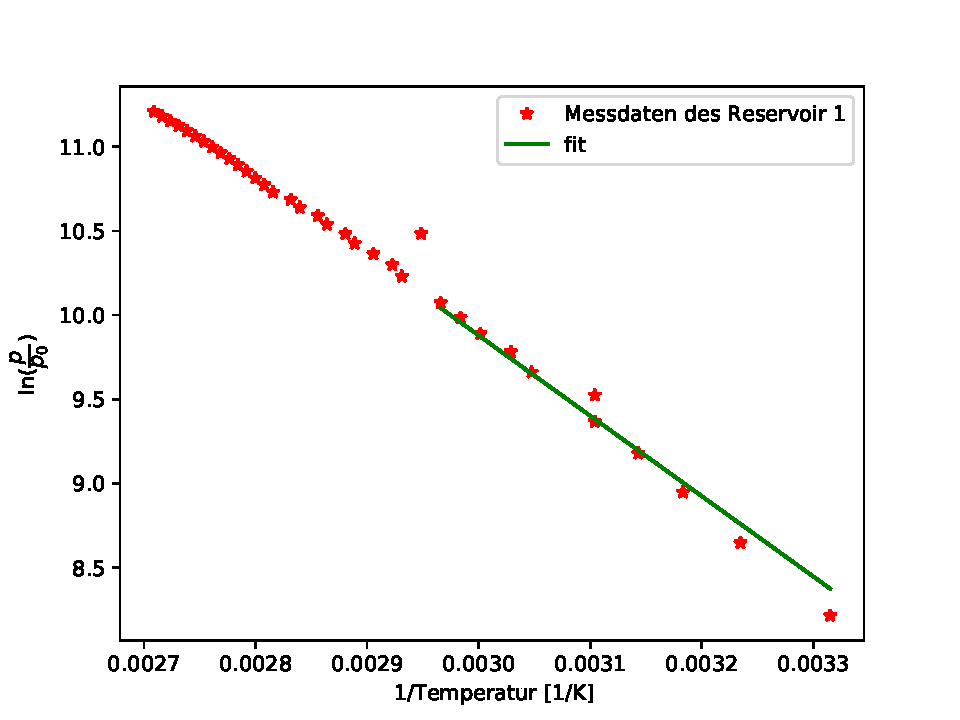
\includegraphics{plot1.pdf}
   \caption{Messwerte und Ausgleichsgerade bis 1 bar}
   \label{fig:plot}
  \end{figure}
  Für die Ausgleichsgerade ergeben sich die Koeffizienten
  \begin{align*}
   a=(-4686.5514 \pm 58.9156)\ K\\
   b=10.1354 \pm 0.2268
  \end{align*}
  Einsetzen in die Formel \eqref{eq:L} liefert:
  \begin{equation*}
    L= - a \cdot R = 39000 \pm 489.85 \dfrac{J}{mol}
  \end{equation*}


